\AddToShipoutPicture{\BackgroundPic}

\chapter{Objetivo}

Jogo de plataforma 2D com elementos de \emph{stealth}, que se passa em um reino de fantasia medieval. A princesa Nadine, personagem principal, tenta recuperar o reino que foi tomado de sua família por um grupo de nobres dissidentes, liderados por Richelieu, um mago poderoso. A princesa deve se manter escondida e iludir seus inimigos para alcançar seu objetivo.

Treinada como uma ladina, Nadine possui uma série de habilidades e itens que a auxiliarão em sua jornada:
\begin{itemize}
	\item {\emph{Rogue Reflex}: caso seja vista por um inimigo, Nadine é capaz de eliminá-lo antes que ele alerte seus aliados;}
	\item {Rolar: Nadine rola no chão para escapar de ataques e evitar ser detectada por inimigos;}
	\item {Movimentação furtiva: como todo bom ladino sabe, o melhor combate é o que não acontece. Nadine se movimenta de maneira furtiva, diminuindo as chances de detecção;}
	\item {Mestra de Poções: Nadine é capaz de fazer diversos tipos de poções para auxiliá-la em seus trabalhos. Alguns tipos são a poção atordoante, explosiva, e de fumaça;}
	\item {Combate: quando não há escapatória e violência é a única maneira, Nadine sabe se cuidar. Apesar de fisicamente frágil, a princesa é capaz de utilizar técnicas letais e não-letais para cuidar de seus inimigos;}
	\item {\emph{Lockpicking}}: Nadine pode utilizar suas ferramentas para abrir qualquer porta em seu caminho;
	\item {Armadilhas: Nadine monta armadilhas para derrotar seus inimigos sem entrar em combate direto;}
	\item {\emph{Pickpocket}: Graças à sua destreza, Nadine consegue roubar itens de inimigos sem que estes percebam.}
\end{itemize}

O jogo possuirá três etapas que terão dificuldade progressiva: Infiltração, Resgate e Confronto.

\begin{itemize}
	\item Na primeira etapa o jogador navegará ambientes externos (Redondezas da Vila, Vila, Portões do Castelo e Fossa) e terá mais oportunidades para exploração vertical.

	\item Na segunda etapa o jogador estará dentro do castelo, passando por ambientes mais fechados (Laboratório, Sala da Guarda, Biblioteca, Torre). A partir de agora o jogador deve utilizar elementos do ambiente para se esconder e técnicas para destrair os inimigos.

	\item A etapa final irá misturar elementos das etapas anteriores e culminará no confronto com o mago. Alguns ambientes dessa etapa podem ser os Aposentos Reais e a Sala do Trono.  
\end{itemize}

O jogo cria o suspense necessário a jogos do gênero \emph{stealth} ocultando ambientes isolados do jogador (por exemplo aqueles do outro lado de uma porta ou parede, ver figura ~\ref{visionmode}). 

	\begin{figure}[h]
		\center
		\subfigure[refreal][Posicionamento real dos personagens]{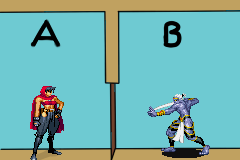
\includegraphics[scale=0.7]{real}}
		\qquad
		\subfigure[refocult][Visão do jogador]{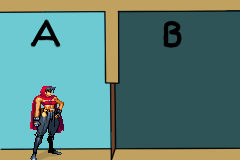
\includegraphics[scale=0.7]{ocult}}
		\caption{Oclusão de Ambiente}
		\label{visionmode}
	\end{figure}

Ao se aproximar de uma porta jogador terá a possibilidade de olhar através da fechadura da mesma para ter uma noção do que o aguarda do outro lado. Nesse modo o jogador terá uma visão em cone da próxima sala, revelando parcialmente o interior da mesma (Figura ~\ref{spy}). Baseado nisso ele poderá escolher entre entrar pela porta ou buscar um meio alternativo que ofereça menos riscos.

Por se tratar de um jogo no qual manter-se oculto é chave, o jogador será capaz de esconder-se atrás de elementos do cenário, como caixas, balcões, árvores ou becos escuros. Também é possível atrair a atenção dos guardas causando perturbações como barulhos, atirando itens do cenário, entre outros.

	\begin{figure}[h!]
		\center
		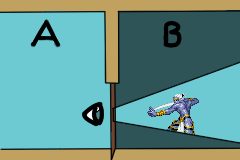
\includegraphics[scale=0.7]{spying}
		\caption{Modo "espião".}
		\label{spy}
	\end{figure}

